These are my lecture notes for Python for Data Analysis, which I consider a work in progress. They're not written to replace class attendance, so you might not find them self-contained. 

The main references for these notes are \cite{lubanovic2019introducing} and \cite{vanderplas2016python}. There are many other fantastic books and resources for self-studying Python. I encourage you to find as many supplementary sources as you find helpful, but to return to these notes to help focus on what will be important for doing well on assignments and exams in this course. 

I've seen this material presented in many different orders. What seems unavoidable in any bearable introduction to Python is that some concept might be slipped in informally before we regroup for a formal explanation of how some data type works or why we keep using words like \emph{object}, \emph{method}, or \emph{callable}. This isn't so different than learning a language through immersion. That's to say we'll be immersed and you might find yourself flipping backwards or forwards in these notes. You could also compare it to bulking and cutting in bodybuilding. Let me know if you see anything that could use restructuring.  

Famous mathematician Paul Halmos counseled students not to study math passively. With Python, this is also good advice. Ease into the language, but don't remain satisfied with running others' code or making only minimal edits. Work from scratch and relish the detours. 

\begin{center}
\href{https://abstrusegoose.com/353}{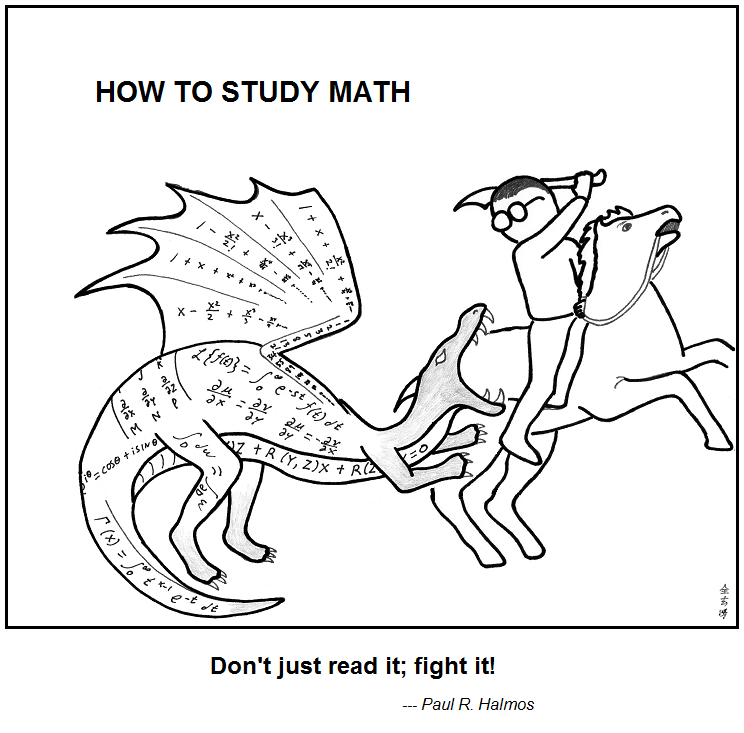
\includegraphics[width = .51\textwidth]{HowMath.png}}

\vspace{-14pt}
\scalebox{0.6}{Source: \link{https://abstrusegoose.com/353}{AbstruseGoose.com}}
\end{center}